\documentclass[11pt,reqno,final]{amsart}

\pdfcompresslevel=0
\pdfobjcompresslevel=0

\usepackage[dvipsnames]{xcolor}% adds colors
\usepackage{amsmath, amsthm}% {amsfonts, amssymb}

% New Characters
\usepackage[latin1]{inputenc}%
\usepackage[T1]{fontenc}

\usepackage{MnSymbol}
\usepackage[normalem]{ulem}% underlining

\usepackage[theoremfont, largesc]{newpxtext} % different text,math font
\usepackage{newpxmath}

\makeatletter
\DeclareMathRadical{\sqrtsign}{symbols}{112}{largesymbols}{112}
\let\sqrt=\undefined
\DeclareRobustCommand\sqrt{\@ifnextchar[\@sqrt{\mathpalette\@x@sqrt}]}
\def\@x@sqrt#1#2{%
 \setbox\z@\hbox{$\m@th#1\sqrtsign{\mkern1mu #2}$}
 \mkern3mu\box\z@}
\makeatother




% Page Typesetting
\usepackage[final]{microtype}
\usepackage{relsize}
\usepackage[margin=1in]{geometry}
\usepackage{framed}
\usepackage{tikz}
\usepackage{setspace}

\usepackage{hyperref}
\hypersetup{
  final,
  pdftitle={Math 135 - Continuity},
  pdfauthor={Bonventre}, 
  linktoc=page,
  pagebackref,
  colorlinks=true,
  citecolor=PineGreen,
  linkcolor=PineGreen,
  linkbordercolor=PineGreen,
}


% Internal References

\usepackage[inline,shortlabels]{enumitem}

\numberwithin{equation}{section} 
\numberwithin{figure}{section}

\usepackage[nameinlink,capitalise,noabbrev]{cleveref}

\crefname{equation}{}{} % get \cref to behave as \eqref

% \theoremstyle{plain} % bold name, italic text
\newtheorem{theorem}[equation]{Theorem}%
\newtheorem*{theorem*}{Theorem}%
\newtheorem{lemma}[equation]{Lemma}%
\newtheorem{proposition}[equation]{Proposition}%
\newtheorem{corollary}[equation]{Corollary}%
\newtheorem{conjecture}[equation]{Conjecture}%
\newtheorem*{conjecture*}{Conjecture}%
\newtheorem{claim}[equation]{Claim}%
\newtheorem{question}{Question}

\theoremstyle{definition} % bold name, plain text
\newtheorem{definition}[equation]{Definition}%
\newtheorem*{definition*}{Definition}%
\newtheorem{example}[equation]{Example}%
\newtheorem*{example*}{Example}%
\newtheorem{remark}[equation]{Remark}%
\newtheorem{notation}[equation]{Notation}%
\newtheorem{convention}[equation]{Convention}%
\newtheorem{assumption}[equation]{Assumption}%
\newtheorem{exercise}[question]{Exercise}

% ---------- macros
\newcommand{\set}[1]{\left\{#1\right\}}%
\newcommand{\sets}[2]{\left\{ #1 \;|\; #2\right\}}%
\newcommand{\longto}{\longrightarrow}%
\newcommand{\into}{\hookrightarrow}%
\newcommand{\onto}{\twoheadrightarrow}%

\usepackage{harpoon}
\newcommand{\vect}[1]{\text{\overrightharp{\ensuremath{#1}}}}

\newcommand{\del}{\partial}%

\newcommand{\ki}{\chi}
\newcommand{\ksi}{\xi}
\newcommand{\Ksi}{\Xi}

\newcommand{\dlim}{\displaystyle\lim}

% %%%%%%%%%%%%%%%%%%%%%%%%%%%%%%%%%%%%%%%%%%%%%%%%%%%%%%%%%%%%%%%%%%%%%%%%%%%%%%%%%%%%%%%%%%%%%%%%%%%%

\begin{document}
\onehalfspacing

\begin{center}
        \textbf{\Large Math 135, Calculus 1, Fall 2020}\\[10pt]
        {\large 09-23: Limits and Continuity}
\end{center}

\thispagestyle{empty}

\renewcommand{\thesection}{\Alph{section}}

\section{Verifying the solutions to 09-21}

Below, we have the answer key to several problems from 09-21. Please provide the correct mathematical reasons/explainations for why these are correct.

Recall that you can only apply the (numbered) Limit Laws when the limits \textbf{exist}.
If any of the limits do not exist, you must use another method to determine the answer (e.g. comparing one-sided limits, calcluating infinite limits, etc).

First, consider the functions $f$ and $g$ from 09-21:
\begin{center}
        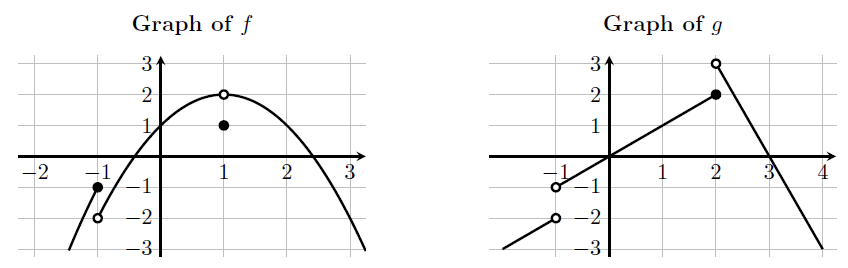
\includegraphics[width=.8\textwidth]{09-23P_graphs.png}
\end{center}

\begin{enumerate}
\item[4.] $\displaystyle\lim_{x \to 2^+}\left( 2\ f(x) + 3 \ g(x) \right) {\color{red} = 11}$
        \vfill
\item[6.] $\dlim_{x \to 2}\left( f(x) - g(x) \right)$ {\color{red} DNE}.\\
        (\textit{Note: it is \textbf{not} sufficient to say that $\dlim_{x \to 2}g(x)$ DNE.})
        \vfill
\item[8.] $\dlim_{x \to 3^+} \dfrac{f(x)}{g(x)} {\color{red} = +\infty}$
        \vfill
\item[11.] $\dlim_{x \to -1}\left( f(x) + g(x) \right) {\color{red} = -3}$.
        \vfill
\end{enumerate}

\newpage
\begin{center}
        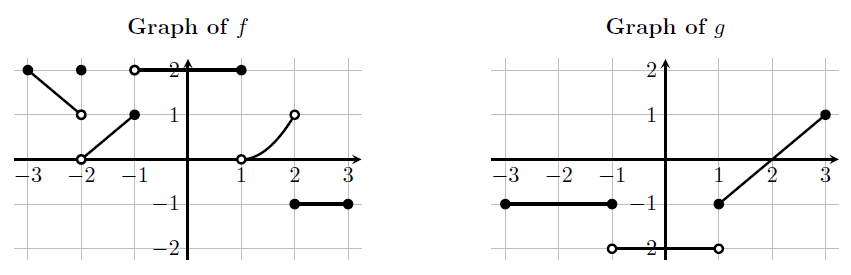
\includegraphics[width=.9\textwidth]{09-23P_graphs2.png}
\end{center}

\begin{enumerate}
\item[7.] $\dlim_{x \to 1^+} f(g(x)) {\color{red} = 2}$
        \vfill
\item[8.] $\dlim_{x \to -2^-} g(f(x)) {\color{red} = -1}$ {\color{red}(and NOT $-2$)}\\
          (\textit{Note: we cannot simply say that% the solution does \textbf{not} depend on a single function value of $g(x)$:
            $\dlim_{x \to -2^-} g(f(x)) = g(\ \dlim_{x \to -2^-} f(x) )$.}
          \vfill
\end{enumerate}

\section{Continuity}

In many of the limit computations from 09-21 and today, the function value and the limit values were different.
This is because, in general, \textit{the function value at $x=a$ has \textbf{no effect} on the limit as $x \to a$ of the function}.

However, some functions are better behaved:
\begin{framed}
        A function $f(x)$ is \textit{continuous at $x=a$} if
        \[
                \dlim_{x \to a} f(x) = f(a).
        \]
\end{framed}

Intuitively:
\begin{itemize}
\item a function is continuous if it can be drawn without having to lift up your pencil.
\item A function is \textit{not} continuous if it has holes, jumps, asymptotes (infinite limits), or places where limits don't exist (e.g. infinite oscillations).
\end{itemize}

There are in fact \textit{three} conditions to check to say that $f(x)$ is continuous at $x=a$:
\begin{enumerate}[(1)]
\item $f(a)$ must exist
\item The limit as $x \to a$ of $f(x)$ must exist (in particular, it cannot be $\infty$ or $-\infty$).
\item The limit must equal the function value.
\end{enumerate}

\newpage

\begin{example}
        Consider the function $f(x)$ on the first page. It is not continuous at $x=-1$ and $x=1$:
        \begin{itemize}
        \item it has a \textbf{jump discontinuity} at $x=-1$: both the left-handed and right-handed limits exist (and are finite), but they are note equal to each other.
        \item it has a \textbf{removable discontinuity} at $x=2$: $\lim_{x \to 1} f(x)$ exists (and equals 2), but this is \textit{different} from the function value $f(1) = 1$.
        \end{itemize}
        However, $f(x)$ is \textbf{left-continuous} at $x=-1$: the left-hand limit exists and equals the function value.
\end{example}

\begin{exercise}
        Is $f(x)$ \textbf{right-continuous} at $x=1$? Why or why not?
        \vfill
\end{exercise}

\begin{exercise}
        Consider the function $h(x)$ with the following graph, and fill in the following table
        (possible types: jump, removable, infinite, other).

        $ $
        \begin{minipage}{.5\textwidth}
                \begin{center}
                        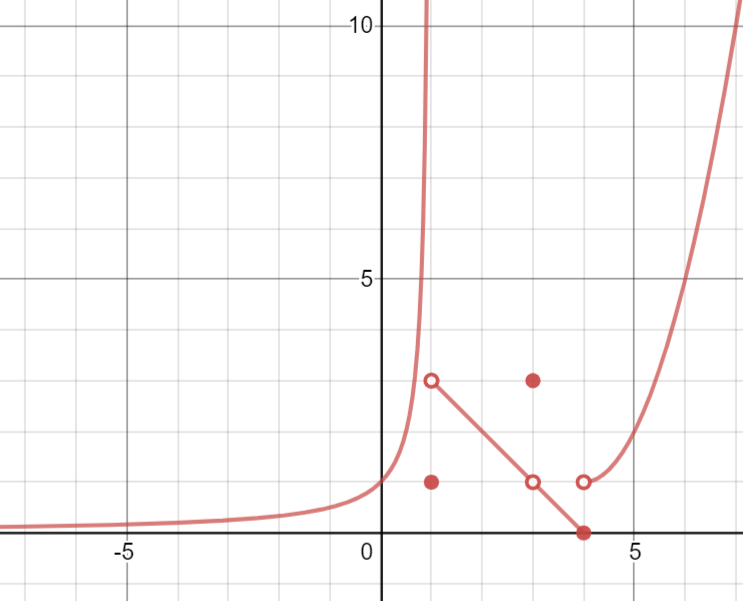
\includegraphics[width=3in]{09-23P_graphs3.png}
                \end{center}
        \end{minipage}
        \begin{minipage}{.5\textwidth}
                {\renewcommand{\arraystretch}{2}%                
                  \begin{center}
                          \begin{tabular}{l|c|c}
                            discontinuity & \quad type \quad $ $& \quad left/right continuous? \\ \hline
                            $x=$ \qquad && \\
                            $x=$ && \\
                            $x=$ && \\ 
                          \end{tabular}
                  \end{center}
                }
        \end{minipage}
\end{exercise}

\begin{framed}
        \begin{itemize}
        \item Polynomials, rational functions, exponentials, logs, trig functions, and algebraic functions are \textit{all continuous on their domains} [See: Limit Law Overview, ``Direct Substitution Property''].
        \item Compositions of continuous functions are continuous.
        \end{itemize}
\end{framed}

To find limits of continuous functions, evaluate the function at the point in question (i.e. just plug it in!).

\begin{exercise}
        Use continuity to find the value of $\dlim_{x \to 3} \log_5(\cos(t-3)+4)$.
        \vfill
\end{exercise}


\end{document}
